\documentclass[10pt]{article}
 
\usepackage[margin=1in]{geometry} 
\usepackage{amsmath,amsthm,amssymb, graphicx, multicol, array}
\usepackage{enumitem}
\usepackage{hyperref}
 
\newcommand{\N}{\mathbb{N}}
\newcommand{\Z}{\mathbb{Z}}
 
\newenvironment{problem}[2][Problem]{\begin{trivlist}
\item[\hskip \labelsep {\bfseries #1}\hskip \labelsep {\bfseries #2.}]}{\end{trivlist}}

\date{Due: Sep 20, 2022 10pm PT}

\begin{document}
 
\title{Assignment 3}
\author{
CS 181AG: Network Algorithmics}
\maketitle

This assignment will give you practice with IP addresses and routing. It includes four questions (no programming this week) and a reading assignment with questions.  

\begin{problem} {1: IP Addresses}
Given the following networks, write the network address, broadcast
address, and the range of hosts in the network.

\begin{enumerate}
    \item 10.1.43.61/29
    \item 192.168.15.33/24
    \item 128.13.0.0/16
    \item Among the three subnets above, which one(s) would have been valid under classful addressing?
    
\end{enumerate}
\subsection*{Answer}
\begin{enumerate}
    \item The network address is $10.1.43.48$, the broadcast address is $10.1.43.63$, and the range of hosts is $10.1.43.49-62$.
    \item THe network address is $192.168.15.0$, the broadcast address is $192.168.15.255$, and the range of host addresses is $ 192.168.15.0-254$.
    \item The network address is $128.13.0.0$, the broadcast address is $128.13.255.255$, and the $128.13.0.1-128.13.255.254$.
    \item The network addresses that would have been valid under classful addressing are numbers 2 and 3 since we have /24 and /16.
\end{enumerate}
\end{problem}
\begin{problem}{2: Longest Matching Prefix}

Suppose a router's forwarding information base contained the following information.
\\\\
\begin{tabular}{|c|c|}
\hline
\textbf{Prefix} & \textbf{Next hop} \\
\hline
192.168.74.0/24 & Router 1 \\
\hline
192.168.74.192/28 & Router 2 \\
\hline
192.168.74.204/30 & Router 3 \\
\hline
10.1.120.0/21 & Router 4 \\
\hline
0.0.0.0/0 & Router 5 \\
\hline
\end{tabular}
\\\\\\
For each of the following IP addresses, where should the router send the packet?
\begin{enumerate}
    \item 192.168.74.198
    \item 192.168.74.207
    \item 10.1.128.12
    \item 192.168.74.208
    \item 10.1.125.74
    \item 192.168.73.0
\end{enumerate}

\subsection*{Answer}
\begin{enumerate}
    \item The router should send the packet to Router 2.
    \item The router should send the packet to Router 3.
    \item The router should send the packet to Router 5.
    \item The router should send the packet to Router 1.
    \item The router should send the packet to Router 4.
    \item The router should send the packet to Router 5.
\end{enumerate}

\end{problem}
\begin{problem}{3: Distance Vector Protocol} Consider running the distance vector protocol on the graph below.

\begin{figure}[h]
    \centering
    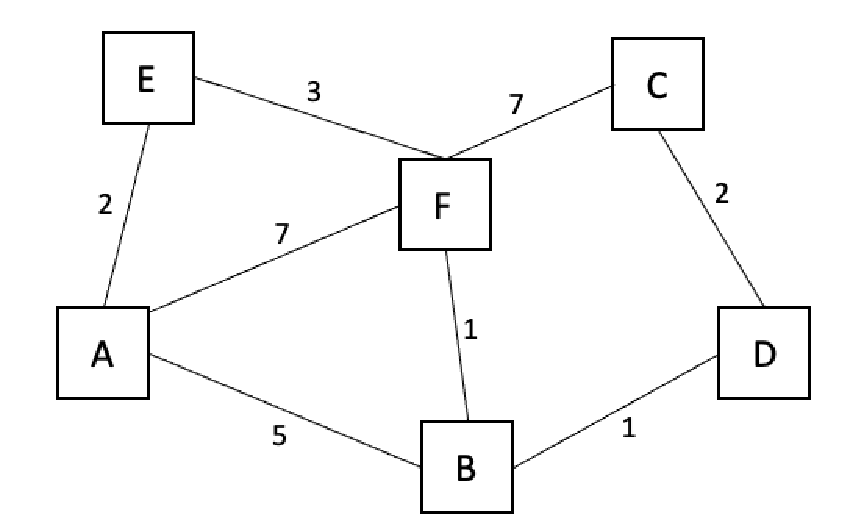
\includegraphics{figures/dvp_graph.pdf}
    \label{fig:dvp}
\end{figure}

The following set of tables show Round 1, where each router only knows about its own neighbors.

\begin{tabular}{|c|c|c|}
\hline
A & 0 & - \\
\hline
B & 5 & B  \\
\hline
C & $\infty$ & -  \\
\hline
D & $\infty$ & -  \\
\hline
E & 2 & E  \\
\hline
F & 7 & F \\
\hline
\end{tabular}
\begin{tabular}{|c|c|c|}
\hline
A & 5 & A \\
\hline
B & 0 & -  \\
\hline
C & $\infty$ & -  \\
\hline
D & 1 & D  \\
\hline
E & $\infty$ & E  \\
\hline
F & 1 & F \\
\hline
\end{tabular}
\begin{tabular}{|c|c|c|}
\hline
A & $\infty$ & - \\
\hline
B & $\infty$ & -  \\
\hline
C & 0 & -  \\
\hline
D & 2 & D  \\
\hline
E & $\infty$ & E  \\
\hline
F & 7 & F \\
\hline
\end{tabular}
\begin{tabular}{|c|c|c|}
\hline
A & $\infty$ & - \\
\hline
B & 1 & B  \\
\hline
C & 2 & C  \\
\hline
D & 0 & -  \\
\hline
E & $\infty$ & E  \\
\hline
F & $\infty$ & F \\
\hline
\end{tabular}
\begin{tabular}{|c|c|c|}
\hline
A & 2 & A \\
\hline
B & $\infty$ & B  \\
\hline
C & $\infty$ & C  \\
\hline
D & $\infty$ & -  \\
\hline
E & 0 & -  \\
\hline
F & 3 & F \\
\hline
\end{tabular}
\begin{tabular}{|c|c|c|}
\hline
A & 7 & A \\
\hline
B & 1 & B  \\
\hline
C & 7 & C  \\
\hline
D & $\infty$ & -  \\
\hline
E & 3 & E  \\
\hline
F & 0 & - \\
\hline
\end{tabular}
\begin{enumerate}
    \item Fill in the next round - you may fill it in here, print and fill, whatever is easiest for you.

Round 2:

\begin{tabular}{|c|c|c|}
\hline
A & 0 & - \\
\hline
B & 5 & B  \\
\hline
C & 14 & F  \\
\hline
D & 6 & B \\
\hline
E & 2 & E \\
\hline
F & 5 & E \\
\hline
\end{tabular}
\begin{tabular}{|c|c|c|}
\hline
A & 5 & A \\
\hline
B & 0 & -   \\
\hline
C & 3 & D \\
\hline
D & 1 & D \\
\hline
E & 4 & F \\
\hline
F & 1 & F \\
\hline
\end{tabular}
\begin{tabular}{|c|c|c|}
\hline
A & 14  & F \\
\hline
B & 3 & D \\
\hline
C & 0 & -  \\
\hline
D & 2 & D \\
\hline
E & 10 & F \\
\hline
F & 7 & F \\
\hline
\end{tabular}
\begin{tabular}{|c|c|c|}
\hline
A & 6 & B \\
\hline
B & 1 & B  \\
\hline
C & 2 & C \\
\hline
D & 0 & -  \\
\hline
E & $\infty$ & - \\
\hline
F & 2 & B \\
\hline
\end{tabular}
\begin{tabular}{|c|c|c|}
\hline
A & 2 & A \\
\hline
B & 4 & F  \\
\hline
C & 10 & F \\
\hline
D & $\infty$ & -  \\
\hline
E & 0 & - \\
\hline
F & 3 & F \\
\hline
\end{tabular}
\begin{tabular}{|c|c|c|}
\hline
A & 5 & E \\
\hline
B & 1 & B  \\
\hline
C & 7 & C  \\
\hline
D & 2 & B  \\
\hline
E & 3 &  E \\
\hline
F & 0 & - \\
\hline
\end{tabular}

\item How many rounds (in total) does the algorithm take to converge?
\end{enumerate}
\subsection*{Answer 3.2}
    It would take 4 rounds in total for the algorithm to converge.

\end{problem}
\begin{problem} {4: Count to Infinity}

Despite being called the count-to-infinity problem, it's possible for the problem to arise without actually counting all the way to infinity. Assuming poison reverse is not being used, consider the following graph and describe a) a sequence of events that could lead to this, and b) how the process would eventually stop. Hint: link changes can be caused by many factors, e.g., broken links, decreased costs, or increased costs

\begin{figure}[h]
    \centering
    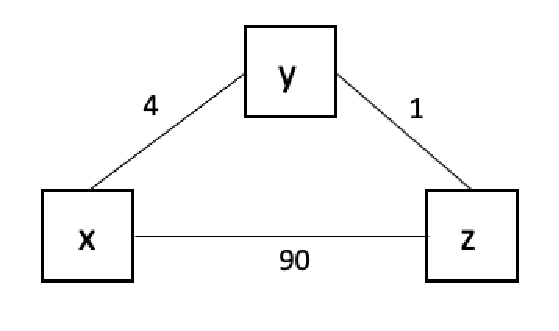
\includegraphics[scale=0.5]{figures/count_inf.pdf}
    \label{fig:count}
\end{figure}

\end{problem}
\subsection*{Answer}
\begin{enumerate}
    \item[(a)] A situation that could lead to the count-to-infinty problem is if the connection between $y$ and $z$ were to be severed as a result of a broken link, as since then, when $x$ sends a message to $z$, it would think that it could do it in $5$, but then $y$, upon recieving the message, would think that it could send a message through $x$ for $9$, leading to the problem at hand.
    \item[(b)] The process would eventually stop when the cost of sending a message to $z$ would be greater than 90 for $x$, as then it would simply use the connection between itself and $z$ to send the message.
\end{enumerate}

\begin{problem}{5: Reading}
In class we learned about IPv4 addresses. Read more about the decades-long effort to switch to IPv6 and the challenges in doing so \href{https://www.potaroo.net/ispcol/2022-05/when.html}{here}. Then answer the following questions. Points are for effort

\begin{enumerate}
    \item Why was IPv6 created? 
    \item What are the main obstacles to moving to IPv6?
\end{enumerate}
\subsection*{Answer}
\begin{enumerate}
    \item IPv6 was created as a response to IPv4's inability to supply enough IP addresses. Due to exponential growth of the internet, the number of hosts would exceed the number of possible hosts in a number of months. Similarly, there were pressures on the routing systems in place where "the deployed routers in 1992 only had enough memory to support a further 12-18 months of routing growth". 
    \item The main obstacles to moving to IPv6 outlined in the paper are resource allocation (focusing more time on meeting the rapid expansion of the internet and on scaling rather than on a way to complete a IPv6 transition), general consensus of use of a decentralized internet (why develop application support if no one is using IPv6, and why use IPv6 if there is no application support for using IPv6 in your tech stack), a poor rep that it recieved due to non-satisfactory methods to ensure compatability between IPv4 and IPv6 (e.g. 6to4), and the fact that the ISP does not support IPv6, nor does IPv6 support any of the IPv6 services that are needed, such as cloud services and cloud platforms.
\end{enumerate}

\end{problem}
\begin{problem}{6}
How long did this assignment take you?
\end{problem}
\subsection*{Answer}
This assignment took me $\approx 5$ hours.

\begin{problem}{7: Extra (optional) reading}
The Internet Engineering Task Force (IETF) was the most prominent group to set internet standards. They did so in the form of Requests for Comments, or RFCs. These tend to be dense with technical specification, but interesting from a historical perspective to understand how each piece of the internet we're learning about was formally proposed and detailed. \href{https://www.rfc-editor.org/rfc/rfc2460}{Here} is the RFC for IPv6. There is no work or credit or extra credit associated with reading this - just more information if it interests you. 
\end{problem}
\end{document}